\section{Results}\label{sec:results}

\subsection{Overall, No Index, 3 Nodes}\label{subsec:overall,NoIndex,3Nodes}
\begin{figure}
    \centering{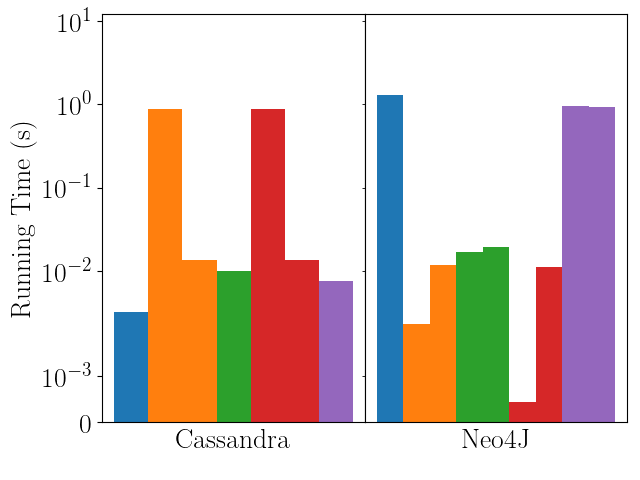
\includegraphics[scale=0.55]{images/qall-3node-none.png}}
    \caption{Running times of different queries for a 3-node Neo4J cluster and a 3-node Cassandra cluster.
    Each point represents the average of 15 runs.
    The blue bars represent query 1, the orange represent queries 2A and 2B, the green represent queries 3
    (Cassandra), 3A, and 3B (Neo4J), the red represents queries 4A and 4B, and the purple represent queries 5
    (Cassandra), 5A, and 5B (Neo4J).}\label{fig:ono3n}
\end{figure}

In~\autoref{fig:ono3n}, all queries are plotted against time for both Neo4J and Cassandra.
Each cluster consists of 3 nodes, and no indexes are applied to any column.

A cursory glance reveals that Neo4J performs better for queries given some position, while
Cassandra performs better when given the \texttt{TYC} ID\@.
Given that the Cassandra families are not indexed by their Equatorial position columns, it makes sense
that Neo4J would shine here.
For queries 2A and 4A, Neo4J performs an average of 0.88s faster than Cassandra.
For queries 1, 3 (3A for Neo4J), and 5 (5A for Neo4J), Cassandra performs an average of 1.13s faster.
Query 3 runs slightly faster on Cassandra than Neo4J, with Cassandra running ~6.7ms faster.

For both Cassandra and Neo4J, queries 2A, 4A and 2B, 4B differ in their approach to determine the region our star is in.
Reading a file containing the region data and determining our \texttt{TYC1} here instead of performing the exhaustive
search on our \textit{Region} family does yield a slight time decrease of 0.46s.
For the non-indexed Neo4J, this approach is instead slightly detrimental to performance (average of 7.5ms increase).
Given that no mechanisms are in place for Neo4J to take advantage of this, it makes sense that no speed up is shown.

In Neo4J queries 5A, 3A, and 5B, 3B, we vary our query to include the \textit{Region} node or not.
Both require a full search of the entire \textit{Star} node list, but the B queries require an additional traversal
to the matching \textit{Region} node and additional hops to each \textit{Star} nodes.
These additional steps suggest that the A queries should be faster, but the results are mixed.
Our results show that queries 3A and 3B are roughly the same (2.7ms difference), while query 5B is actually ~39ms
faster than 5A\@.
There appears to be some Neo4J optimization for queries using relationships.

For singular element searches, our 3 node Cassandra cluster performs seconds faster than our non-indexed Neo4J cluster.
If we are not given a star ID, then Neo4J performs slightly faster by tenths of a second.
In terms of query time distribution, the average deviation of all Cassandra queries is 0.139s while
the average Neo4J deviation is 1.75s.
Neo4J queries can take up to 2 minutes to return a result, and under a second for others.

%Part of this may be due to Neo4J's partition intolerance, where dropped or delayed messages lead a long waiting
%period.

On average, our Cassandra cluster performs all queries faster than our non-indexed Neo4J cluster by 0.1s.

\subsection{Queries \{1, 3, 5\}, TYC Index, 3 Nodes}\label{subsec:queries1,3,5,TycIndex,3Nodes}
\begin{figure}
    \centering{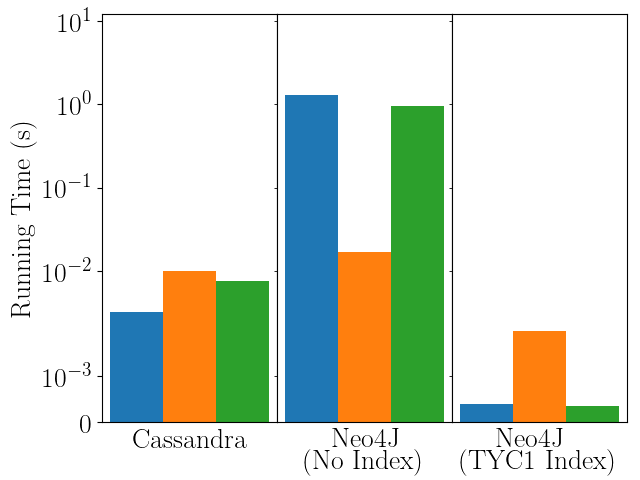
\includegraphics[scale=0.55]{images/q135-3node-tycindex.png}}
    \caption{Running times of queries 1, 3, and 5 for a 3-node Cassandra cluster, a 3-node Neo4J cluster without an
    index on \texttt{TYC1}, and another 3-node Neo4J cluster with the specified index.
    Each point represents the average of 15 runs.
    The blue bars represents query 1, the orange represents query 3 (3A for Neo4J), and the green represents query 5
    (5A for Neo4J).}\label{fig:1qtycindex3n}
\end{figure}

In~\autoref{fig:1qtycindex3n}, queries 1, 3 (3A for Neo4J), and 5 (5A for Neo4J) are plotted for a Cassandra cluster,
a Neo4J cluster without any indexes, and a Neo4J cluster with an index on \texttt{TYC1}.
All of three of these queries involve searching for some star based on the \texttt{TYC1} field.

On average, a properly indexed Neo4J cluster (on \texttt{TYC1}) performs slightly faster than Cassandra by ~6ms.
Cassandra performs 0.75s faster than a non-indexed Neo4J cluster.
The average difference in time between a non-indexed Neo4J cluster and the indexed Neo4J cluster is 0.76s.
A slight performance boost may be gained for both Neo4J query 1s if a size restriction filter were placed (i.e.
\texttt{LIMIT}).
For the non-indexed case, this query is of complexity $T(n) = \Theta(n)$ and could be lowered to $O(n)$ if we
restrict our resultant to one element.

It's interesting to note that query 3A for the non-indexed Neo4J cluster was already fast relatively to
queries 1 and 5A (~17ms vs. average of 1.14s).
All queries involve iterating through the entire \textit{Star} node set, yet relaxing the
\texttt{TYC2} and \texttt{TYC3} constraints results in a faster query.

\subsection{Queries \{4, 5\}, TYC \& BTmag Index, 3 Nodes}\label{subsec:queries4,5,TycbtmagIndex,3Nodes}
\begin{figure}
    \centering{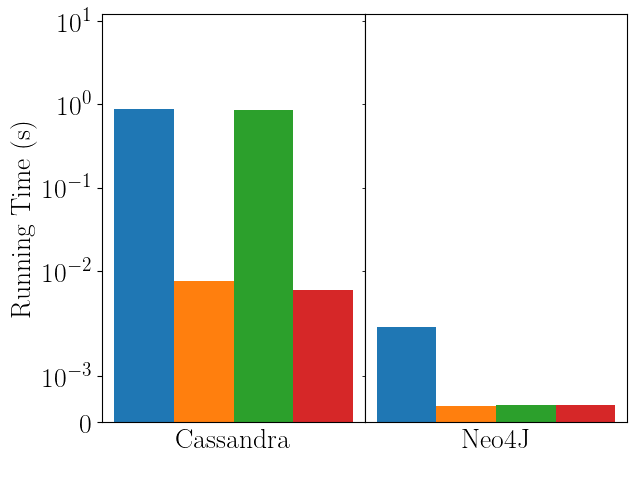
\includegraphics[scale=0.55]{images/q45-3node-bttycindex.png}}
    \caption{Running times of queries 4 and 5 for a 3-node Cassandra cluster with an without an index on \texttt{BTmag},
    a 3-node Neo4J cluster with an index on \texttt{TYC}, and another with an index on both \texttt{TYC} and
    \texttt{BTmag}.
    Each point represents the average of 15 runs.
    The blue bars represent queries 4A without the \texttt{BTmag} index, the orange represents query 5 (5A for Neo4J)
    without the \texttt{BTmag} index, the green represents queries 4A with the index, and the red represents query 5
    (5A for Neo4J) with the index.}\label{fig:45qtycbti3}
\end{figure}

In~\autoref{fig:45qtycbti3}, queries 4A and 5 (5A for Neo4J) are plotted for a Cassandra and Neo4J 3-node cluster
with and without an index on \texttt{BTmag}.
Both of these queries involve searching for nearby stars and applying a brightness restriction filter.

Neo4J with the appropriate \texttt{TYC} indexes performs queries 4 and 5 ~0.22s faster than Cassandra, regardless of
the additional \texttt{BTmag} index or not.
Cassandra experiences a slight increase in speed (~13ms on average), suggesting Cassandra's QEP (query execution
planner) does take advantage of the index.
The current Neo4J cluster performs the same with or without the \texttt{BTmag} index for both queries (1.6ms difference
on average).
Results may differ for the Neo4J case if the \texttt{TYC} indexes were not already applied, which might have showed
a greater impact with and without the \texttt{BTmag} index.

\subsection{Query 1, TYC \& BTmag Index, 1--3 Nodes}\label{subsec:queries1,2,TycbtmagIndex,1-3Nodes}
\begin{figure}
    \centering{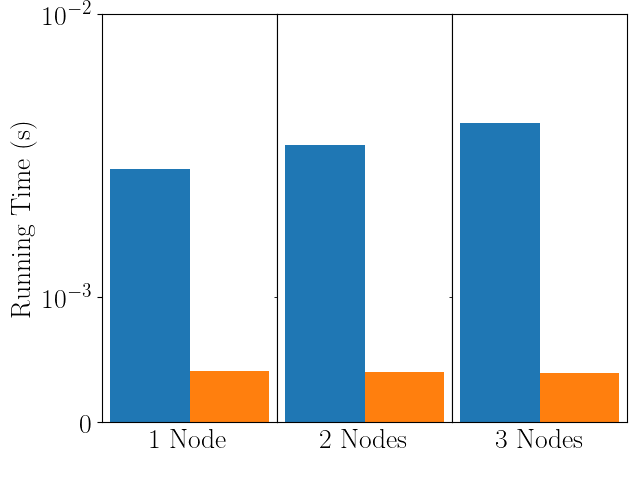
\includegraphics[scale=0.55]{images/q1-123node-none.png}}
    \caption{Running times of query 1 for 1--3 node Cassandra and Neo4J clusters.
    All Neo4J clusters have an index on \texttt{TYC1}.
    The blue bars represent the Cassandra queries, while the orange represent the Neo4J queries.
    Each point represents the average of 15 runs.}\label{fig:1qtyc123}
\end{figure}

In ~\autoref{fig:1qtyc123}, query 1 is plotted for Cassandra and Neo4J clusters of varying node size (1 to 3 nodes).


